\onecolumn
\chapter{Auswertung}
\label{ch:auswertung}

\section*{Fehlerrechnung}
Für die statistische Auswertung von $n$ Messwerten $x_i$ werden folgende Größen definiert \cite{errorSkript25}:
\begin{align}
    \bar{x} &= \frac{1}{n} \sum_{i=1}^{n} x_i \vphantom{\sqrt{\sum_i^n}^2} && \text{\textcolor{gray}{Arithmetisches Mittel}} \label{eq:arithmetisches_mittel} \\
    \sigma^2 &= \frac{1}{n-1} \sum_{i=1}^{n} (x_i - \bar{x})^2 \vphantom{\sqrt{\sum_i^n}^2} && \text{\textcolor{gray}{Variation}} \label{eq:variation} \\
    \sigma &= \sqrt{\frac{1}{n-1} \sum_{i=1}^{n} (x_i - \bar{x})^2} \vphantom{\sqrt{\sum_i^n}^2} && \text{\textcolor{gray}{Standardabweichung}} \label{eq:standardabweichung} \\
    \Delta \bar{x} &= \frac{\sigma}{\sqrt{n}} = \sqrt{\frac{1}{n(n-1)} \sum_{i=1}^n(\bar x - x_i)^2} \vphantom{\sqrt{\sum_i^n}^2} && \text{\textcolor{gray}{Fehler des Mittelwerts}} \label{eq:fehler_mittelwert} \\
    \Delta f &= \sqrt{\left(\frac{\partial f}{\partial x} \Delta x\right)^2 + \left(\frac{\partial f}{\partial y} \Delta y\right)^2} \vphantom{\sqrt{\sum_i^n}^2} && \text{\textcolor{gray}{Gauß’sches Fehlerfortpflanzungsgesetz für $f(x,y)$}} \label{eq:gauss_fehlfortpflanzung} \\
    \Delta f &= \sqrt{(\Delta x)^2 + (\Delta y)^2} \vphantom{\sqrt{\sum_i^n}^2} && \text{\textcolor{gray}{Fehler für $f = x + y$}} \label{eq:fehler_summe} \\
    \Delta f &= |a| \Delta x \vphantom{\sqrt{\sum_i^n}^2} && \text{\textcolor{gray}{Fehler für $f = ax$}} \label{eq:fehler_proportional} \\
    \frac{\Delta f}{|f|} &= \sqrt{\left(\frac{\Delta x}{x}\right)^2 + \left(\frac{\Delta y}{y}\right)^2} \vphantom{\sqrt{\sum_i^n}^2} && \text{\textcolor{gray}{relativer Fehler für $f = xy$ oder $f = x/y$}} \label{eq:relativer_fehler} \\
    \sigma &= \frac{|a_{lit} - a_{gem}|}{\sqrt{\Delta a_{lit}^2 + \Delta a_{gem}^2}} \vphantom{\sqrt{\sum_i^n}^2} && \text{\textcolor{gray}{Berechnung der signifikanten Abweichung}} \label{eq:signifikante_abweichung}
\end{align}

\twocolumn



\section{Bestimmung der Brennweite der achromatischen Linse}
\label{sec:auswertung_brennweite_achromat}

\begin{table*}[t!]
    \centering
    \begin{tabular}{l | c c c c | c c}
        \hline
        Beziehung $f$ zu $g$ & $g \,[\mathrm{cm}]$ & $b \,[\mathrm{cm}]$ & $B \,[\mathrm{cm}]$ & $\beta$ & Art & Richtung \\
        \hline
        $\infty > g > 2f$ & $25,00 \pm 0,05$ & $16,50 \pm 0,05$ & $0,30 \pm 0,05$ & $0,660 \pm 0,024$ \\
        & $30,00 \pm 0,05$ & $15,00 \pm 0,05$ & $0,20 \pm 0,05$ & $0,500 \pm 0,019$ & reel & umgekehrt  \\
        & $35,00 \pm 0,05$ & $14,00 \pm 0,05$ & $0,20 \pm 0,05$ & $0,400 \pm 0,015$ \\
        \midrule
        $g = 2f$ & $18,90 \pm 0,05$ & $19,00 \pm 0,05$ & $0,40 \pm 0,05$ & $1,01 \pm 0,04$ & reel & umgekehrt \\
        \midrule
        $2f > g > f$ & $15,00 \pm 0,05$ & $27,10 \pm 0,05$ & $0,70 \pm 0,05$ & $1,81 \pm 0,07$ \\
        & $12,50 \pm 0,05$ & $31,90 \pm 0,05$ & $0,90 \pm 0,05$ & $2,552 \pm 0,110$ & reel & umgekehrt  \\
        & $10,50 \pm 0,05$ & $46,50 \pm 0,05$ & $1,30 \pm 0,05$ & $4,429 \pm 0,216$ \\
        \midrule
        $g = f$ & $9,90 \pm 0,05$ & - & - & - & kein Bild \\
        \midrule
        $f > g > 0$ & $8,00 \pm 0,05$ & - & - & - & virtuell & aufrecht \\
        \bottomrule
    \end{tabular}
    \caption{Messwerte der Beziehung zwischen $f$ und $g$. Die Gegenstandsgröße wurde auf $G = 0{,}8 \pm 0{,}05\,\mathrm{cm}$ vermessen.}
    \label{tab:messwerte_achromat}
\end{table*}

Die Messwerte zur Bestimmung der Brennweite der achromatischen Linse sind aus Tabelle 1 des \hyperref[Protokoll]{Protokolls} entnommen. Aus den Messwerten für Gegenstandsweite $g$ und Bildweite $b$ wurde jeweils der Abbildungsmaßstab $\beta$ nach \hyperref[eq:abbildungsmassstab]{Gleichung \ref*{eq:abbildungsmassstab}} berechnet. Die Gegenstandsgröße wurde auf $G = 0{,}8 \pm 0{,}05\,\mathrm{cm}$ vermessen. Der Fehler von $\beta$ wurde über \hyperref[eq:gauss_fehlfortpflanzung]{Gauß'sch Fehlerfortpflanzung (\ref*{eq:gauss_fehlfortpflanzung})} bestimmt:
\begin{equation}
    \Delta \beta = \sqrt{\left(\frac{1}{g} \Delta b\right)^2 + \left(\frac{b}{g^2} \Delta g\right)^2}.
\end{equation}

Die Ergebnisse sind in Tabelle 1 zusammengefasst. Die Brennweite $f$ wurde für jede Messung über \hyperref[eq:linsengleichung]{Gleichung \ref*{eq:linsengleichung}} berechnet. Sen Fehler berechnet sich zu:
\begin{equation}
    \Delta f = \frac{1}{(b+g)}\sqrt{\left(b^2 \cdot \Delta g\right)^2 + \left(g^2 \cdot \Delta b\right)^2}.
\end{equation}

Über diese Gleichungen und den Messwerten der Tabelle 1 des \hyperref[Protokoll]{Protokolles} ergeben sich die Werte der \hyperref[tab:messwerte_achromat]{Tabelle \ref*{tab:messwerte_achromat}}.

Die Ergebnisse für $g=f$ und $f>g$  werden nicht aufgelistet, da diese kein Bild erzeugen, welches vermessen werden kann. Für $g=f$ liegt das Bild im Unendlichen und für $f>g$ entsteht ein virtuelles, aufrechtes Bild, welches sich nicht auf einem Schirm abbilden lässt.

In er Tabelle sind auch die qualitativen Beobachtungen gelistet. das virtuelle Bild, welches Aufrichtig ist, konnte so nicht wirklich beobachtet werden, dies ist die theoretische Beobachtung. Das $\beta$ für $g > 2f$ ist kleiner als 1, was bedeutet, dass das Bild kleiner als der Gegenstand ist. Für $g = 2f$ ist das Bild genauso groß wie der Gegenstand ($\beta \approx 1$). Für $f < g < 2f$ ist das Bild größer als der Geg enstand ($\beta > 1$).

Die Abbildungen für die verschiedenen Bereiche der Gegenstandsweite $g$ sind in \hyperref[fig:auswertung_achromat1]{Abbildung \ref*{fig:auswertung_achromat1}} skizziert. 
Aus der Tabelle 1 des \hyperref[Protokoll]{Protokolls} wurden die Bildweiten gegen die Gegenstandsweiten in \hyperref[fig:auswertung_achromat2]{Abbildung \ref*{fig:auswertung_achromat2}} aufgetragen. Die Schnittpunkte der Geraden sollten die Brennweite der Linse ergeben. Leider sind die Messwerte sehr streuend, was auf eine ungenaue Messung der Gegenstands- und Bildweiten hindeutet. Wo genau der Fehler liegt, ist nicht klar. Die \hyperref[fig:auswertung_achromat3]{Abbildungen \ref*{fig:auswertung_achromat3}, \ref*{fig:auswertung_achromat4}} zeigen die gleichen Messwerte, jedoch wurden in \hyperref[fig:auswertung_achromat3]{Abbildung \ref*{fig:auswertung_achromat3}} die Geraden so angepasst, dass die Gegenstandsweiten als korrekt angenommen wurden. In \hyperref[fig:auswertung_achromat4]{Abbildung \ref*{fig:auswertung_achromat4}} wurden die Geraden so angepasst, dass die Bildweiten als korrekt angenommen wurden. In \hyperref[fig:auswertung_achromat5]{Abbildung \ref*{fig:auswertung_achromat5}} wurden alle Geraden übereinander gelegt. 

Die \hyperref[tab:vergleich_g_b]{Tabelle \ref*{tab:vergleich_g_b}} zeigt, dassdie Abweichungnen der Gegenstandsweiten im Durchschnitt kleiner sind als die der Bildweiten. Besonders, wenn die Gegendstandweite klein ist. Dies deutet darauf hin, dass die Bildweiten ungenauer gemessen wurden. Dies könnte daran liegen, dass das Bild unscharf war und es schwierig war, den genauen Punkt zu bestimmen, an dem das Bild scharf ist. Für große gegenstandsweiten sind beide Messwerte relativ genau. Die Abweichungen sind in \hyperref[tab:vergleich_g_b]{Tabelle \ref*{tab:vergleich_g_b}} zusammengefasst. Die Abweichungen sind als absoluter und relativer Fehler angegeben. Der relative Fehler ist in Klammern angegeben.


\begin{table*}[h!]
    \centering
    \caption{Vergleich zwischen tatsächlichen und bestimmten Werten von $g$ und $b$.}
    \begin{tabular}{c c c c c c}
        \hline
        $g_{gem}$ [cm] &  $b_{gem}$ [cm] & $b_{bes}$ [cm] & $g_{bes}$ [cm] & \cellcolor{red!10}Abweichung $g$ [cm] & \cellcolor{red!10}Abweichung $b$ [cm] \\
        \hline
        10,5 & 46,5 & >100 & 12,8 & \cellcolor{red!10}$2,3 (21,9\%) $& \cellcolor{red!10} $\min -50$ \\
        12,5 & 50,0 & 31,9 & 14,6 & \cellcolor{red!10}$2,1 (16,8\%)$ & \cellcolor{red!10}-18,1 (36,2\%) \\
        15,0 & 30,0 & 27,1 & 15,7 & \cellcolor{red!10}$0,7 (4,7 \%)$ & \cellcolor{red!10}-2,9 (9,7\%)\\
        18,9 & 21,2 & 19,0 & 21,0 & \cellcolor{red!10}$2,1 (11,1\%)$ & \cellcolor{red!10}-2,2 (10,4\%)\\
        25,0 & 16,5 & 16,5 & 25,2 & \cellcolor{red!10}0,2 (0,8\% ) & \cellcolor{red!10}0,0 \\
        30,0 & 15,0 & 15,0 & 29,6 & \cellcolor{red!10}-0,4 (1,3\%) & \cellcolor{red!10}0,0 \\
        35,0 & 14,0 & 14,0 & 35,0 & \cellcolor{red!10}0,0  (0\%  ) & \cellcolor{red!10}0,0 \\
        \hline
    \end{tabular}
    \label{tab:vergleich_g_b}
\end{table*}

\onecolumn
\begin{figure}[h!]
    \centering
    \includegraphics[width=\textwidth, page=4]{Protokolle/31/Chapter/Messprotokoll.pdf}
    \caption{Skizzen der Versuchsaufbauten und der Strahlenverläufe für die verschiedenen Bereiche der Gegenstandsweite $g$.}
    \label{fig:auswertung_achromat1}
\end{figure}

\begin{figure}[h!]
    \centering
    \includegraphics[width=\textwidth, page=5]{Protokolle/31/Chapter/Messprotokoll.pdf}
    \caption{Bild- gegen Gegendstandweite. Schnittpunkt aller Graden sollte die Brennweite der Linse ergeben.}
    \label{fig:auswertung_achromat2}
\end{figure}

\begin{figure}[h!]
    \centering
    \includegraphics[width=\textwidth, page=6]{Protokolle/31/Chapter/Messprotokoll.pdf}
    \caption{Bild- gegen Gegendstandweite. Grün sind der Sollwert der Brennweite, wie sie im Versuch bestimmt wurde. Rot sind die Geraden unter annahme, dass die gegenstandsweiten korrekt bestimmt wurden.}
    \label{fig:auswertung_achromat3}
\end{figure}

\begin{figure}[h!]
    \centering
    \includegraphics[width=\textwidth, page=7]{Protokolle/31/Chapter/Messprotokoll.pdf}
    \caption{Bild- gegen Gegendstandweite. Grün sind der Sollwert der Brennweite, wie sie im Versuch bestimmt wurde. Lila die Geraden unter annahme, dass die Bildweiten korrekt bestimmt wurden.}
    \label{fig:auswertung_achromat4}
\end{figure}

\begin{figure}[h!]
    \centering
    \includegraphics[width=\textwidth, page=8]{Protokolle/31/Chapter/Messprotokoll.pdf}
    \caption{Bild- gegen Gegendstandweite. Überlagerung aller Geraden. Blau sind die tatsächlichen Geraden, Rot die Geraden unter annahme, dass die gegenstandsweiten korrekt bestimmt wurden. Lila die Geraden unter annahme, dass die Bildweiten korrekt bestimmt wurden.}
    \label{fig:auswertung_achromat5}
\end{figure}

\twocolumn

\section{Brennweitenbestimmung der bikonvexen Linse nach Bessel}
\label{sec:auswertung_brennweite_bikonvex}
In diesem Abschnitt soll die Brennweite der bikonvexen Linse $L_1$ mit dem Bessel-Verfahren bestimmt werden. Die Messwerte sind in Tabelle 2 des \hyperref[Protokoll]{Protokolls} zu finden. Der Abstand zwischen Gegenstand und Schirm wurde auf $L = 60 \pm 0{,}1\,\mathrm{cm}$ eingestellt. Die Positionen der Linse für die scharfe Abbildung wurden notiert, woraus sich die Abstände $d$ der beiden Positionen berechnen lassen. Es wird der Mittelwert der Messreihe gebildet und sein Fehler auf \hyperref[eq:fehler_mittelwert]{Fehler des Mittelwerts (\ref*{eq:fehler_mittelwert})} geschätzt. Zudem soll der Ablesefehler beider Messugnen zu einerm gesamten verechnet werden. Die Brennweite wurde dann über \hyperref[eq:bessel]{Gleichung \ref*{eq:bessel}} berechnet. Der Fehler wurde über \hyperref[eq:gauss_fehlfortpflanzung]{Gauß'sches Fehlerfortpflanzungsgesetz (\ref*{eq:gauss_fehlfortpflanzung})} bestimmt:
\begin{equation}
    \Delta f = \sqrt{\left(\frac{L^2 + d^2}{4L^2} \Delta L\right)^2 + \left(\frac{d}{2L} \Delta d\right)^2}.
\end{equation}

Die Ungenauigkeit von $d$ ist die kombination aus dem statistischem Fehler des Mittelwerts und dem Ablesefehler. Es ergibt sich:
\begin{equation}
    \Delta d = \sqrt{(\Delta d_{stat})^2 + (\Delta d_{abg})^2},
\end{equation}

Daraus ergibt sich für der Abstand $d$:
\begin{equation}
    \underline{
        d = 26{,}20 \pm 0{,}18\,\mathrm{cm}.
    }
\end{equation}

Aus dieser lässt sich nun die Brennweite berechnen:
\begin{equation}
    \boxed{
        f = (12{,}13 \pm 0{,}05)\,\mathrm{cm}.
    }
\end{equation}

Angegeben war eine Brennweite von $f_{lit} = 12\,\mathrm{cm}$. Die Abweichung beträgt somit:
\begin{equation}
    \frac{\left| f - 12 \, \mathrm{cm} \right|}{\Delta f} = 0,26\sigma,
\end{equation}
Somit konnte die Brennweite der Linse mit dem Bessel-Verfahren sehr genau bestimmt werden und die Herstellerangaben bestätigt werden. Die Abweichung scheint somit rein statistisch zu sein.

\section{chromatische und sphärische Aberration}
\label{sec:auswertung_aberration}
Die Messwerte zur Untersuchung der chromatischen und sphärischen Aberration sind in den Tabellen 3 und 4 des \hyperref[Protokoll]{Protokolls} zu finden. Die Messung der Brennweite wurde mit einem Rot- und einem Blaufilter wiederholt, um die chromatische Aberration zu untersuchen. Zusätzlich wurde die Linse einmal mit einer Lochblende und einmal mit einer Ringblende betrieben, um den Einfluss der sphärischen Aberration auf die Brennweite zu beobachten. Veränderungen des Abstandes $d$ zwischen den Bessel-Positionen deuten auf Unterschiede in der effektiven Brennweite hin. Der Abstand zwischen Gegenstand und Schirm wurde auf $L = 60 \pm 0{,}1\,\mathrm{cm}$ eingestellt. Die Positionen der Linse für die scharfe Abbildung wurden notiert, woraus sich die Abstände $d$ der beiden Positionen berechnen lassen. Es wird der Mittelwert der Messreihe gebildet und sein Fehler auf \hyperref[eq:fehler_mittelwert]{Fehler des Mittelwerts (\ref*{eq:fehler_mittelwert})} geschätzt. Zudem soll der Ablesefehler beider Messugnen zu einerm gesamten verechnet werden. Die Brennweite wurde dann über \hyperref[eq:bessel]{Gleichung \ref*{eq:bessel}} berechnet. Der Fehler wurde über \hyperref[eq:gauss_fehlfortpflanzung]{Gauß'sches Fehlerfortpflanzungsgesetz (\ref*{eq:gauss_fehlfortpflanzung})} bestimmt und sind analog zu Abschnitt \ref{sec:auswertung_brennweite_bikonvex}. 
Die Ergebnisse sind in \hyperref[tab:messwerte_aberration]{Tabelle \ref*{tab:messwerte_aberration}} zusammengefasst.
\begin{table}[!ht]
    \centering
    \begin{tabular}{l | c c | c}
        \hline
        Messung & $d \,[\mathrm{cm}]$ & $f \,[\mathrm{cm}]$ & Abw. $f$ \\
        \hline
        ohne Blende & $26{,}20 \pm 0{,}18$ & $12{,}13 \pm 0{,}05$ & - \\
        \midrule
        Lochblende & $24{,}80 \pm 0{,}10$ & $12{,}437 \pm 0{,}028$ & $10,6\sigma$ \\
        Ringblende & $26{,}20 \pm 0{,}10$ & $12{,}140 \pm 0{,}028$ & $ < 0,01\sigma$ \\
        \midrule
        Rotfilter & $27{,}0 \pm 0{,}3$ & $11{,}97 \pm 0{,}08$ & $2,17\sigma$ \\
        Blaufilter & $27{,}7 \pm 0{,}4$ & $11{,}81 \pm 0{,}10$ & $3,44\sigma$ \\
        \hline
    \end{tabular}
    \caption{Messwerte zur Untersuchung der chromatischen und sphärischen Aberration.}
    \label{tab:messwerte_aberration}
\end{table}

Anhand der Tabellenwerte lässti sich erkennen, das mit ausnahme der Ringblende alle Messungen eine signifikante Abweichung zur Messung ohne Blende aufweisen. Die Lochblende hat die Brennweite auf $f = 12{,}437 \pm 0{,}028\,\mathrm{cm}$ erhöht. Dies ist darauf zurückzuführen, dass die Lochblende nur achsennahe Strahlen durchlässt, welche eine längere Brennweite haben. Die Ringblende hingegen lässt nur Strahlen durch, die weit von der optischen Achse entfernt sind. Diese haben eine kürzere Brennweite, welche jedoch in diesem Fall nicht signifikant von der Messung ohne Blende abweicht. 
Die Brennweite beim roten Licht ist größer als die vom blauen Licht. Somit lässt sich vermuten, dass eine größere Wellenlänge zu einer größeren Brennweite führt. Dies ist darauf zurückzuführen, dass rotes Licht weniger stark gebrochen wird als blaues Licht. Die Abweichung der beiden Brennpunkte liegt bei $1,25\sigma$, was auf eine signifikante Abweichung hindeutet.

\section{Untersuchung des Gitters}
\label{sec:auswertung_mikroskop}

Es wurde ein Gitter mithilfe eines Mikroskopes untersucht. Als Objekt diente ein Kreuzgitter-Dia, welches hinter einer Lampe mit Grünfilter positioniert wurde. Das Zwischenbild wurde in einem definierten Abstand zur Objektivlinse auf einem Schirm abgebildet, der eine Millimeterskala trug. Hinter dem Zwischenbild wurde das Okular in seiner Brennweite positioniert, sodass das Auge auf unendlich akkommodierte. Die Vergrößerung wurde aus der Gitterstruktur des Zwischenbilds bestimmt. Anschließend wurde der einstellbare Spalt schrittweise verengt, bis die vertikalen Strukturen des Gitters gerade nicht mehr aufgelöst werden konnten. Aus der Spaltbreite und dem Abstand zum Objekt wurde der Öffnungswinkel berechnet, aus dem sich mit \hyperref[eq:auflösung]{Gleichung \ref*{eq:auflösung}} das Auflösungsvermögen ergab. Der Versuch wurde mit rotem und blauem Licht wiederholt, um den Einfluss der Wellenlänge auf die Auflösung zu überprüfen.

\subsection{Gitterkonstante}
\label{ssec:gitter}
Zunächst wurde die Gitterkonstante des Kreuzgitters bestimmt. Huerzu muss seine Breite $b_G$ bestimmt werden. Über eine Abzählung wurde bestimmt, dass die Breite von 10 Gitterlinien $b_{10} = 5{,}0\,\mathrm{mm}$ beträgt. Daraus ergibt sich die Breite einer Gitterlinie zu:
\begin{equation}
    b_G = \frac{b_{10}}{10} = 0{,}50\,\mathrm{mm}.
\end{equation}

Der Fheler von $b_G$ berehcnet sich über \hyperref[eq:fehler_proportional]{Gleichung \ref*{eq:fehler_proportional}}. Es wird ein Ablesefehler von $\Delta b_{10} = 0{,}1\,\mathrm{mm}$ angenommen. Somit ergibt sich:
\begin{equation}
    \Delta b_G = \frac{b_{10}}{10^2} \Delta b_{10} = 0{,}007\,\mathrm{mm}.
\end{equation}

wobei $\Delta b_{10} = \sqrt{2 \cdot 0,1^2}$ der Ablesefehler ist. Somit ergibt sich für die Gitterbreite:
\begin{equation}
    \boxed{
        b_G = (0{,}500 \pm 0{,}007)\,\mathrm{mm}.
    }
\end{equation}

Aus der Gitterbreite lässt sich die Gitterkonstante $G$ bestimmen:
\begin{equation}
    G = \frac{b_G}{\beta}.
\end{equation}

Dabei ist $\beta$ der Abbildungsmaßstab des Mikroskops. Dieser wird über
\begin{equation}
    \beta = \frac{b}{f_1} - 1
\end{equation}

bestimmt. Mit $b = 25{,}0 \pm 0{,}1\,\mathrm{cm}$ als Abstand zwischen Objektiv und Zwischenbild und $f_1 = 10{,}0 \pm 0{,}1\,\mathrm{cm}$ als Brennweite des Objektivs. Der Fehler von $\beta$ berechnet sich über \hyperref[eq:gauss_fehlfortpflanzung]{Gauß'sches Fehlerfortpflanzungsgesetz (\ref*{eq:gauss_fehlfortpflanzung})} zu:
\begin{equation}
    \Delta \beta = \sqrt{\left(\frac{1}{f_1} \Delta b\right)^2 + \left(\frac{b}{f_1^2} \Delta f_1\right)^2}.
\end{equation}

Somit ergibt sich für den Abbildungsmaßstab:
\begin{equation}
    \underline{
        \beta = 5{,}25 \pm 0{,}16.
    }
\end{equation}

Der Fehler der Gitterkonstante berechnet sich über \hyperref[eq:gauss_fehlfortpflanzung]{Gauß'sches Fehlerfortpflanzungsgesetz (\ref*{eq:gauss_fehlfortpflanzung})} zu:
\begin{equation}
    \Delta G = \sqrt{\left(\frac{1}{\beta} \Delta b_G\right)^2 + \left(\frac{b_G}{\beta^2} \Delta \beta\right)^2}.
\end{equation}  

Somit ergibt sich für die Gitterkonstante:
\begin{equation}
    \boxed{
        G = (0{,}095 \pm 0{,}003)\,\mathrm{mm}.
    }
\end{equation}

\subsection{Auflösungsvermögen}
\label{ssec:aufloesung}

Anschließend wurde der einstellbare Spalt schrittweise verengt, bis die vertikalen Strukturen des Gitters gerade nicht mehr aufgelöst werden konnten. Die Messwerte sind in Tabelle 5 des \hyperref[Protokoll]{Protokolls} zu finden. Das \hyperref[eq:arithmetisches_mittel]{Arithmetisches Mittel (\ref*{eq:arithmetisches_mittel})} und sein Fehler sind somit:
\begin{equation}
    D = (4,00 \pm 0,17) cm
\end{equation}

Im \hyperref[Protokoll]{Messprotokoll} ist der Abstand zwischen Gitter und Spalt $s = (4,3 \pm 0,1) cm$ vermerkt. Aus diesen beiden Werten lässt sich der Minimalöffnungwinkel $varphi$ bestimmen:
\begin{equation}
    \varphi = \arctan \left(\frac{D}{2s}\right) 
\end{equation}

Über die \hyperref[eq:gauss_fehlfortpflanzung]{Gauß'sche Fehlerfortpflanzung (\ref*{eq:gauss_fehlfortpflanzung})} lässt sich der Fehler zu
\begin{equation}
    \Delta \varphi = \frac{1}{\left(\frac{D}{2s}\right)^2 + 1} \sqrt{\left(\frac{1}{2s} \Delta D\right)^2 + \left(\frac{D}{2s^2} \Delta s\right)^2}
\end{equation}

Damit ist der Winkel:
\begin{equation}
\boxed{
    \varphi = (0,44 \pm 0,04) rad
}
\end{equation}

Nach \hyperref[eq:auflösung]{Gleichung \ref*{eq:auflösung}} und einer Wellenlänge von grünem Licht $\lambda_g = 550nm$, sowie $n=1$, da das Medium Luft ist. Der Fehler nach \hyperref[eq:gauss_fehlfortpflanzung]{Gauß'scher Fehlerfortpflanzung (\ref*{eq:gauss_fehlfortpflanzung})} bestimtm sich zu:
\begin{equation}
    \Delta G_{min} = 0,61 \cdot \frac{\lambda \cdot \cos\varphi}{\sin^2\varphi} \cdot \Delta \varphi
\end{equation}

Daraus ergibt sich
\begin{equation}
    G_{min} = (790 \pm 70) nm
\end{equation}

Die \hyperref[eq:auflösung]{Gleichung \ref*{eq:auflösung}} it zudem stringent mir der Beobachtung, dass bei blauem Licht die Auflösung geringer ist, während sie bei rotem Licht größer wird. Dies hängt mit der Wellenlänge zusammen.

\subsection*{Uneinigkeiten}

Vergleicht man die Ergebnisse des der Gitterkonstante aus \ref{ssec:gitter} und \ref{ssec:aufloesung}, so kommen uneinigkeiten auf:
\begin{equation}
 \frac{\left| G - G_{min} \right|}{\sqrt{(\Delta G)^2 + (\Delta G_{min}^2)}} = 31,39\sigma
\end{equation}

Dies sill in der \hyperref[ch:diskussion]{Diskussion \ref*{ch:diskussion}} genauer betrachet werden.